% Chapter Template

\chapter{Binary Code Profiling} % Main chapter title

\label{c:prof} % Change X to a consecutive number; for referencing this chapter elsewhere, use \ref{ChapterX}

%----------------------------------------------------------------------------------------
%	SECTION 1
%----------------------------------------------------------------------------------------
\section{IPET Analysis}
The WCET for a function is calculated using implicit path enumeration technique (IPET) \cite{li1995performance}. IPET is a method of pessimistically determining the longest execution path of a program without having to enumerate all paths. The first step is to convert the control flow graph (CFG) of a program into an integer linear program (ILP) and the second step is to approximate the cost (i.e. execution time) of each basic block using microarchitectural modelling and/or dataflow analysis. 

The goal of the ILP is to maximize the objective function:

\begin{equation}
\sum_{i=1}^{N}c_ix_i
\end{equation}

where:

\begin{itemize}
  \item $N$: Number of basic blocks
  \item $c_i$: Execution time of block $i$
  \item $x_i$: frequency of block $i$
\end{itemize}

The CFG is transformed into a set of linear constraints by noting that the number of times a basic block is entered must equal the number of times it is exited. Each edge in the CFG is assigned a variable $e_i$. The entry edge into the root basic block has the constraint $e_0 = 1$. For all other edges, constraints are extracted based on the observation that for each basic block: $\sum e_{in} - \sum e_{out} = 0$. For example, in Figure~\ref{f:bbedges}: $e_0+e_1+e_2-e_3=0$.

\begin{figure}[h]
\centering
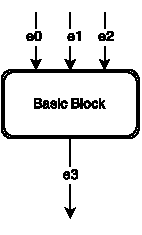
\includegraphics[scale=1]{bbedges.pdf}
\caption{Sum of the edges into the basic block must equal the sum of the edges out: $\sum e_{in} - \sum e_{out} = 0$.} 
\label{f:bbedges}
\end{figure}


% Loops require an additional constraint on the maximum number of times the loop can can run. Therefore for each loop $\sum e_{in} \leq m$ where $m$ is the maximum number of iterations. In Figure~\ref{f:loopedges}, taking $m=10$ gives: $e_0 + e_1 + e_2 + e_4 \leq 10$. Functions calls are not explicitly represented in the constraint system. Each function is analyzed independently and then the final execution time of a basic block $i$ that calls function $f$ is defined as: 
%   $(c_i+WCET(f))x_i$. Recursive function calls are not supported but are also generally not used in real-time systems.


Loops require an additional constraint on the maximum number of iterations. Therefore for each loop $\sum e_{in} - \sum \mathrm{maxIter}*e_{fl} \le 0$, where $\mathrm{maxIter}$ is the maximum number of iterations for the loop and $e_{fl}$ are the non-backwards edges into the loop (i.e. those that can only execute once per single round of loop iterations).


\begin{figure}[h]
\centering
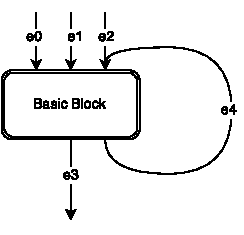
\includegraphics[scale=1]{loopedges.pdf}
\caption{An additional constraint is required for loops: $\sum e_{in} \leq m$.} 
\label{f:loopedges}
\end{figure}


The entry-point for function calls equals the sum of all the edges leaving basic blocks that call that function. In Figure~\ref{f:function-ipet}, the result is: $e_2+e_3-e_4 = 0$. 

\begin{figure}[h]
\centering
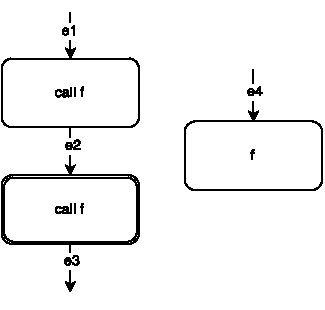
\includegraphics[scale=1]{function-ipet.pdf}
\caption{The sum edges leaving function call blocks is equal to the edge entering that function's root block.} 
\label{f:function-ipet}
\end{figure}
 

\section{Building CFG and Loop Detection}
	Inspired by Heptane \cite{heptane}, the tool uses \texttt{objdump} to disassemble the compiled elf file for analysis. 
	The initial parsing phase examines each instruction to categorize each line of assembly code (e.g. store, branch). 
	First, a list of functions and their contained code is built. Second, the code is divided into a list of basic blocks (i.e. block of code with one entry point and one exit point). 
	Branches, jumps, and call instructions are used as endpoints of a basic block. 
	The destinations of branches and calls are then identified to split basic blocks containing destination points into two separate blocks. 
	Each basic block object has references to its successor and predecessor blocks.

	Loop detection takes place once the CFG is constructed. 
	First, the \emph{rank} of each basic block is determined using Algorithm~\ref{a:rank}. 
	Loops are then detected by identifying a backwards edge between basic blocks. 
	The predecessor of a backwards edge has a higher rank than the successor.

\begin{algorithm}

\SetKwFunction{setRank}{setRank}

root.age $\leftarrow$ 1\;
mark root as seen\;
bbList $\leftarrow$ list of basic blocks\;
bbList.add(root);
setRank(2,root,bbList)\;

\Fn{\setRank{int rank,BasicBlock bb, list bbList}}{
	\For{all successor $b_s$ of bb}{
		\If{bbList does not contain $b_s$ and $b_s.rank < bb.rank$}{
			$b_s.rank$ = rank\;
			bbList.add($b_s$)\;
			setRank(rank+1,bbList)\;
			bbList.remove($b_s$)\;
		}
	}
}
\caption{Basic block rank calculation for CFG}
\label{a:rank}
\end{algorithm}

Annotations on maximum loop iterations can be embedded in the binary using the following macro \cite{heptane}:

\includecode{annot.h}{l:annot}{C macro to include loop annotations in program binary}{C}

	Inline assembly supports labels assigned only number names that do not have to be unique in the program (but do have to be unique to the inlined code). 
	References to the label must indicate whether they are forwards (f) or backwards (b). 
	This code defines a label, and then writes a reference to that label (address) and the number 1 to the section \texttt{.wcet\_annot}. 
	The contents of the annotation section can be extracted and parsed with \texttt{objdump} as well.



% 
% The pre-existing intermediate representation (IR) is a basic control flow graph (CFG) constructed from the assembly code. The structure of the IR and tools is shown in Figure~\ref{f:class}. Basic blocks have been identified and the instruction types have been roughly categorized (e.g. branch, binary operation). However, the operation and operands are still in unparsed string form. Before loop analysis can be done, several steps must be taken to create a more meaningful IR for the code within basic blocks.

% \addfigure{0.55}{class.pdf}{Class diagram of profiling tool}{f:class}

\section{Static Analysis}

\subsection{Analysis Framework}

	Typical program analyses is implemented using an iterative fixed point procedure. 
	The analysis will propagate information through the CFG until a fixed point is reached. Each analysis can be defined in terms of several general patterns, coloquially referred to as ``Laurie's six steps'' \cite{lauriesteps}. 
	First, the approximation produced by an analysis must be well defined. 
	Second, an analysis is defined as either \emph{forwards}, where information is propagated down through the CFG from predecessor to successor, and \emph{backwards} analysis, where information is propagated from successor to predecessor. 
	Third, a merge operation must be defined for join points in the CFG. 
	Fourth, the behaviour of the analysis must be defined for each type program statement in terms of the in-set and out-set of each basic block. Generally, the analysis will remove (kill) some members of the inset and add some new members to the out-set(gen). The gen and kill for each program statement will depend on the in set as well as the type of statement. 
	Finally, the starting values for either the in or out set of every basic block must be defined (depending on whether the analysis is forwards or backwards). Generally, the in values are the same for all nodes except, possibly, for the start node.

	A framework architecture is used to define a generic \emph{forward analysis} procedure that is extended to implement specific analyses. The framework is currently limited to intraprocedural analysis. The framework implements a worklist based approach for fixed point flow analysis \cite{andrew2002modern}.

\addfigure{0.6}{stages.pdf}{Stages of loop analysis}{f:stages}
	We wish to use static analysis to automatically generate constraints on the program without the use of source code annotations.
	The CFG described above is not sufficient to do static analysis on the program. 
	The assembly representation of the basic blocks must be transformed into a higher level intermediate representation (IR). 
	Standard compiler techniques \cite{andrew2002modern} are used to build larger expressions out of the assembly instructions, perform substitutions, and simplify expressions in order to determine properties of the program semantics. 

	The analysis stages are shown in Figure~\ref{f:stages}. 
	The first three stages (dominance frontier, phi insertion and variable renaming) are standard steps in transforming code into static single assignment (SSA) form. 
	SSA form creates a new variable name every time a new value is assigned rather than reuse the same variable names. 
	Therefore, each variable in the program only has one definition which simplifies many analyses.
	
	
	After transforming the program into SSA form, Reaching expressions analysis, loop analysis, and branch analysis are used to automatically generate constraints for IPET analysis. 
	Reaching expression analysis builds a list of available expressions at each program point p and automatically substitutes any variables with unambiguous values. 
	Afterwards, loop analysis determines the loop induction variable and the maximum number of iterations for a loop. 
	Branch analysis determines the maximum number of times a branch within a loop may execute if its condition depends on the induction variable.

\subsection{Static Single Assignment}
	
	The first step in transforming the program into SSA is to compute the dominance frontier. 
	A node $d$ strictly dominates another node $n$ if all paths from the start node to $n$ go through $d$. 
	An immediate dominator \emph{idom} of a node n is the \emph{unique} node that dominates $n$ but does not dominate any of the other dominator nodes of $n$. 
	The dominance frontier of node $d$ is the set of nodes $n$ where $d$ dominates an immediate predecessor of $n$ but does not strictly dominate $n$. 
	
	The second step in transforming the program into SSA is to insert $\phi$ functions. A $\phi$ function explicitly represents a merge operation for different values a variable may have when a basic block has several successors. For instance, consider the following code:
	
	\begin{lstlisting}
	if(x > 0) y = 5;
	else y = 100;
	//program point p
	\end{lstlisting}
	
	In SSA form there two possible reaching definitions of the variable \texttt{y} to consider at program point p. 
	To resolve this conflict, a \texttt{phi} function is inserted that represents the merge of the values ($y_3 = \phi(y_1,y_2)$).

	Finally, the variables are renamed by assigning an increasing number to each definition of a variable. 
	A sample input and output are shown in Listing~\ref{l:ssa-example}. One detail worth mentioning is that function calls cause an increment to the counter of the return registers $r_2$ and $r_3$.
	Algorithmic details are provided in \cite{andrew2002modern}.
	

\begin{figure}[h]
\captionsetup{type=lstlisting}
\caption{Example of SSA renaming output}
\begin{sublstlisting}[t]{0.47\linewidth}
\caption{Original Code}
\lstinputlisting[captionpos=t,language=C]{code/ssa.c}
\end{sublstlisting} \hfill
\begin{sublstlisting}[t]{0.47\linewidth}
\caption{Renamed Code}
\lstinputlisting[captionpos=t,language=C]{code/ssa.s}
\end{sublstlisting}
\label{l:ssa-example}
\end{figure}




\subsection{Reaching Expression Analysis}

The reaching expression analysis combines elements of reaching defintion analysis, constant propagation and copy propagation. The analysis is defined by the following six properties:

\begin{enumerate}
  \item The analysis approximates lists of expressions that may be available on the stack or in registers.
  \item At a program point $p$, we would like to know the expressions that \textit{may} be stored on the stack or in registers.  We would also like to substitute older expressions into newer expressions as they are generated at each $p$ during the analysis if the substitution is \textit{unambiguous} (i.e. if only one definition is reaching).
  \item This is a forwards analysis.
  \item The merge operation is a simple union. 
  \item In general, registers and frame offsets will be considered temporary variables and the entire frame offset (e.g. ``-8(fp)'') will be considered an identifier. The frame pointer can safely be considered a constant value for intraprocedural analysis as it is only modified in the prologue and epilogue.
   
  \textbf{loads}: $out(S) = (in(S) - kill(S)) \cap gen(S)$ where the kill set is any previous expression stored in the destination register and the generated value is either the identifier of the load source or the expression that was stored there if it was known. 
  
  \textbf{moves}: same as load.
  
  \textbf{stores}: $out(S) = (in(S) - kill(S)) \cap gen(S)$ where the kill set is any previous expression stored in the destination address and the generated value is either the identifier of the source register or the expression that was stored there if it was known.
  
  \textbf{binary operators}: $out(S) = (in(S) - kill(S)) \cap gen(S)$ where the kill set is any previous expression stored in the destination register and the generated expression corresponds to the condition of the instruction.
  
  \textbf{conditional branches}: The expression evaluated by conditional branches are useful state to propagate for the loop analysis but is not stored on the stack or in a register. The expression is placed in the out set at a key corresponding to the instruction address.
  
  \textbf{$\phi$ function}: The merge operation combines sets of expressions from different branches. The $\phi$ function explicitly handles the merges of different versions of the same variable. For example $\phi(a_3) \leftarrow a_2,a_1$ generates the set $\{a_3, \{in(a_2) \cup in(a_1)\}\}$. The $\phi$ function kills the sets for $a_2$ and $a_1$.
  
  All other expressions have no effect at the current time. Support for more statement types will be added as necessary. Function calls do not currently kill the values of return registers however they do increment the counter of the return registers in the variable renaming stage. The flow contains a few extra terms due to this limitation.
  
  \item As this is a \textit{may} analysis, $in(start)=\{\}$ and $in(s)=\{\}$. 
\end{enumerate}

An exerpt from the analysis output is shown in Listing~\ref{l:reachexp}. The example shows how expressions are constructed and how known old values of variables are immediately folded into newer ones. The $\phi$ function merges the expressions from the previous definitions into the new one and kills the old references. It is also possible to maintain a symbol table of definitions. The definition of a variable can be unambiguously retrieved since there is only one. Definitions can be conveniently retrieved for variables that have already beek killed in the flow-set for the current line of code when attempting to simplify expressions later on in the loop analysis.

\begin{lstlisting}[caption={Example reaching expression analysis},label=l:reachexp,captionpos=t]
Basic block start address: 10e0
@!Address: 10e0; instruction: movhi; operands: r3_1,0@!
in: {}
out: {r3_1=[(0) << (16)]}
-------------------------------
@!Address: 10e4; instruction: addi; operands: r3_2,r3_1,9248@!
in: {r3_1=[(0) << (16)]}
out: {r3_2=[((0) << (16)) + (9248)], r3_1=[(0) << (16)]}
-------------------------------
@!Address: 10e8; instruction: mov; operands: r2_1,zero@!
in: {r3_2=[((0) << (16)) + (9248)], r3_1=[(0) << (16)]}
out: {r3_2=[((0) << (16)) + (9248)], r2_1=[0], r3_1=[(0) << (16)]}
-------------------------------
@!Address: 10ec; instruction: movi; operands: r4_1,300@!
in: {r3_2=[((0) << (16)) + (9248)], r2_1=[0], r3_1=[(0) << (16)]}
out: {r3_2=[((0) << (16)) + (9248)], r2_1=[0], r3_1=[(0) << (16)], r4_1=[300]}
-------------------------------
****************************************************
Basic block start address: 10f0
@!Address: 10f0; instruction: phi; operands: r3_2,r3_4 -> r3_3@!
in: {r3_3=[], r3_2=[((0) << (16)) + (9248)], r3_4=[(r3_3) + (24), (((0) << (16)) + (9248)) + (24)], ...}
out: {r3_3=[((0) << (16)) + (9248), (r3_3) + (24), (((0) << (16)) + (9248)) + (24)], ...}

\end{lstlisting} 

\subsection{Loop Analysis}

Algorithm~\ref{a:analysis} shows how the loop is characterized. Note that nested loops do not break the condition that only one backwards edge can exist because a backwards edge is defined as going back to the \textit{head} of the loop. 

The maximum number of iterations of a loop $l$, defined as $M(l)$, is given by the following equation:
\begin{equation}
	M(l) = 
	\begin{dcases*}
		\max{\left \lceil \frac{threshold - initial}{increment} \right \rceil}, & $\{<,>\}$ expressions \\
		\max{\left \lceil \frac{threshold - initial + 1}{increment} \right \rceil}, & $\{\leq,\geq\}$ expressions
	\end{dcases*}
	\label{eq:max}
\end{equation}
and subject to the constraints:
\begin{equation}
(\min(th) > \max(init)) \wedge (\min(inc) > 0), \{<,\leq\} \text{expressions} 
\end{equation}
\begin{equation}
(\max(th) < \min(init)) \wedge (\max(inc) < 0), \{>,\geq\} \text{expressions} 
\end{equation}
Zero and infinite iterations throw exceptions for now. All values in all ranges must respect constraints.
		
The maximum or minimum of each range is chosen as appropriate to maximize $M(l)$.	

	
\begin{algorithm}
\KwData{Function f}
\KwResult{Max iteration for each loop in f}
reachingExp = Reaching expression analysis on f\;
\Begin{
	\For{Loop l in f.getLoops()}{
		String iterator; \tcp{Name of induction variable} \
		Range incrValue; \tcp{Range of values for constant increment} \
		Range threshold; \tcp{Range of constant threshold for loop exit} \
		Range initValue; \tcp{Range of constant initial values for induction} \
		BasicBlock $backEdge\leftarrow$getSingleBackwardsEdge(l)\;
		\If{backEdge == null}{
			fail\;		}
		BasicBlock $exitPoint\leftarrow$getSingleExitPoint(l)\;
		\If{exitPoint == null}{
			fail\;
		}
		conditionOut $\leftarrow$ The reaching expressions at $exitPoint$\;
		branchCondition $\leftarrow$ The expression of the branch condition in $conditionOut$\;
		Simplify $branchCondition$\;
		$iterator \leftarrow$ lefmost identifier in $branchCondition$\;
		\tcp{tricky part} \
		Find expressions $thresholdExp$ and $initExp$\;
		$inSet \leftarrow $ merged output of $\phi(iterator)$ without backwards edge\;
		\If{$inSet$ contains non-constant expressions}{
			\If{inSet.size() $>$ 1}{
				fail \tcp{limit one common unkown for now}
			}
			remove common unknown identifier from $thresholdExp$ and $initExp$\;
		}
		determine ranges from expressions\;
		\If{all ranges defined}{
			$l.maxIterations \leftarrow$ getMaxIterations(initValue,threshold,incrValue,branchCondition.type)\;
		}\Else {
			fail\;
		}
	}
}
 
 \caption{Algorithm for loop analysis.}
 \label{a:analysis}
 \end{algorithm}
 
 \begin{algorithm}
 
\SetKwFunction{getRange}{getRange}
  \SetKwProg{Fn}{Function}{}{}
  \Fn{\getRange{expList}}{
	  $Range \leftarrow$ null\;
	  \For{$exp$ in $expList$}{
	  	\If{$exp$ is binary operation}{
	  		$exp \leftarrow$ simplify $exp$
	  	}
	  	\If{$exp$ is constant}{
	  		$value \leftarrow$ $exp.value$\;
	  		\If{$range$ is null}{
	  			$range \leftarrow [value,value]$\;
	  		}\Else{
	  			\If{$value < range.min$}{
	  				$range.min \leftarrow value$\;
	  			}\ElseIf{$value > range.max$}{
	  				$range.max \leftarrow value$\;
	  			}
	  		}
	  	}
	  	\Else{
	  		\Return null\;
	  	}
	  }
	  \Return $range$\;
  }
  \caption{Get range function for loop detection.}
 \end{algorithm}




\subsection{Example}
It may be easier to demonstrate the behaviour of the analysis with an example. Consider the code in Listing~\ref{l:matmul} and corresponding CFG in Figure~\ref{f:matmul}. This function is interesting because there is nested looping, the inner loops use the array address as induction variables in the assembly code, and the number of iterations can be calculated despite the fact that the initial array address is unknown.

The analysis does not examine the loops in any specific order. The middle-level loop beginning at 0x17a4 is first. The branch condition is then identified (line 4). When the branch condition takes this form then the threshold and increment can be easily identified (lines 7 and 8). The initial condition is also found and the maximum iterations is calculated (lines 9 to 14). The second loop is a bit tricker because the initial value and threshold are offset by a constant unkown (lines 23 and 25). This pattern is recognized by the analysis and the unkown term is cancelled out from both expressions (lines 26 to 29).

\subsection{Conditional branches Depending on Induction Variable}
The expressions for conditional branches inside the body of a loop (that are not the backwards or exit edges) may be checked to see if they depend on the induction variable.The maximum number of times the true branch is taken can then be calculated using Equation~\ref{eq:max} with same increment value and updated threshold and initial values that reflect the condition. For example, a conditional branch with expression \texttt{if(i > 75)} contained in a loop \texttt{for(i = 0; i < 100; i++)} will execute a maximum of 24 times using Equation~\ref{eq:max} with an initial value of 76 and threshold of 100.
 
\begin{lstlisting}[caption={Example output for loop analysis on matrix multiplication code.},label={l:matmul-out},captionpos=t]
loop head: 17a4; tail: 17e0; body: 17a4, 17e0, 17bc,
exit point: BB @17e0
backwards edge head: BB @17e0
branch condition: ((r9_3) + (1)) != (128)
simplified lhs: (r9_3) + (1)
iterator: r9_3
increment: [1]
threshold: [128]
merged inSet: [0]
initial value = [0]
thresholdRange = [128,128]
incrementRange = [1,1]
initialRange = [0,0]
maxIterations = 128
//Second loop *************
loop head: 17bc; tail: 17bc; body: 17bc,
exit point: BB @17bc
backwards edge head: BB @17bc
branch condition: ((r2_4) + (4)) != (r8_2)
simplified lhs: (r2_4) + (4)
iterator: r2_4
increment: [4]
threshold: [r8_2]
merged inSet: [(r8_2) + (-512)]
initial value = [[(r8_2) + (-512)]]
Initial value not constant!
Matching unknown in threshold and initial: r8_2
new initial value: [-512]
new threshold: [0]
thresholdRange = [0,0]
incrementRange = [4,4]
initialRange = [-512,-512]
maxIterations = 128
...
\end{lstlisting}


\printCode{matmul}{Example for loop analysis}{l:matmul}
% \includecode{matmul.c}{l:matmul}{Example code for loop analysis}{C}
\addfigure{0.7}{matmul.pdf}{CFG for matrix multiplication example in Listing~\ref{l:matmul}}{f:matmul}


\section{Validation}
\subsection{Static Analysis}
28 micro-benchmarks were used to test the various forms a loop may have (see Appendix~\ref{A:ProfBench}). The benchmarks are fairly representative of the different forms a loop may take. All benchmarks pass that meet the general pattern outlined in this report. Listing~\ref{l:fail} shows one case that does not work when compiling without optimizations. The analysis only considers the behaviour of the variable in the loop condition and fails to recognize that $x$ is in fact behaving as an induction variable and that $k$ depends on $x$. Interestingly, gcc optimizes out the variable $k$ with -O so a more generic analysis of conditional expressions may improve the loop analysis.

\begin{lstlisting}[caption={Indirect test on induction variable fails.},label=l:fail]
int g8 (){

	int k = 1;
	int x = 0;
	while(k == 1){
		if(x == 105){
			k = 0;
		}
		x++;
		a[x] = x;
	}
	return x;
}
\end{lstlisting}

The matrix multiplication example is one of the benchmarks used in the WCET Workshop competition. Listing~\ref{l:inter} shows a useful case from another benchmark that fails without interprocedural analysis. A summary approach could be used to identify that the missing information is a function argument. However, this information is not easily integrated into the ILP formulation (which I've decided not to discuss in this report). Control flow representing infeasible paths is also generally difficult and requires several ILP problems to be generated representing sets of orthogonal constraints in the solution space. Function pointers are another interesting case that require interprocedural analysis.

\begin{lstlisting}[caption={Interprocedural analysis is necessary to analyze programs that call a function which takes the threshold as an argument.},label={l:inter}]
uint8_t fixFilter(uint8_t *f, int size){
  int i;
  int length = 1 << size;
  int sum = 0;
  for(i = 0; i < length; i++){
    sum = sum + f[i];	
  }   
  // divide by length
  sum = sum >> size;
  return sum;
}
\end{lstlisting}

The maximum number of iterations for each loop is checked by the test framework. The total number of instructions generated by the ILP solver is checked against an instruction accurate simulator. 

Infeasible path detection is a third area of interest where interprocedural analysis could also be of value. For example, in Listing~\ref{l:inter}, it is not possible for both \texttt{g()} and texttt{h()} to be executed. The current analysis does not recognize that both conditions cannot be true in the same pass. There is plenty of existing work on infeasible paths and IPET \cite{gustafsson2006automatic,suhendra2006efficient}.


\begin{lstlisting}[caption={Infeasible path analysis is required to further tighten the WCET estimates.},label={l:inter}]
void paths(x){
	if(x > 0){
		g() //expensive function
	}
	//... later on, x not redefined
	if(x < 0){
		h() //another expensive function
	}
}
\end{lstlisting}


The Malarden benchmarks~\cite{gustafsson2010malardalen} as well as PapaBench~\cite{nemer2006papabench} are often used in work on WCET profiling. This tool should be capable of handling these benchmarks largely without annotations once some form of interprocedural analysis and infeasible path detection are in place. It may be necessary to generate several sets of constraints and iterate over several ILP solutions if the flow information becomes too complex 




\subsection{IPET Validation}

The results of the static analysis and annotations where the analysis still fails can be checked against the instruction accurate simulation of the function. The predicted number of instructions matches the prediction exactly when the analysis is sufficiently robust to represent the nuances of the control flow. We are thus confident that the analysis has been properly implemented. However, the real challenge and art comes in determining cycle accurate response times.

There are some limitations on the IPET analysis. First, recursive functions cannot be analyzed. Any handling of recursive functions will require interprocedural analysis with dynamic call graph generation. A second related issue, pointer analysis is required to determine function pointer targets and build full call graphs. 



Library functions, especially software implemented floating point operations, can also be difficult to analyze. They contain many branches to targets stored in registers making it difficult to build a complete CFG (much like the function pointer except the targets may (or may not) be in the same function body). As a result, some measurement based approximations are used for library functions. Currently, only a subset of floating point operations have been analyzed.


Floating point behaviour is approximated by observing the number of times a loop executed in an OVP simulation environment over several thousand random inputs in the range $[-1000,1000]$. The observed worst case number of loop executions is then used to generate constraints when a floating point operation is encountered in a program. The measured number of instructions are not used because in future work it may still be desirable to analyze the entire floating point function using michro-architectural modelling in which case the number of instructions will not be sufficient. Indirect jump destinations are simply ignored. 

Figure~\ref{f:ipetresults} shows the WCET calculated using IPET normalized to the measured execution time (maximum number of instructions observed in OVP) for all four operations. Single-precision is tested without integer multiplication hardware (SP-SW). Double precision is tested with integer multiplication hardware (DP-SW-I) and without (DP-SW). This chart demonstrates that software-based floating point operations are a source of imprecision that is difficult to overcome. Note that there is no guarantee that this is in fact an \emph{over}-estimate because it is not clear that the inputs tested in fact yield the worst case path (although it is likely an over-estimate).

\begin{figure}[h]
\centering
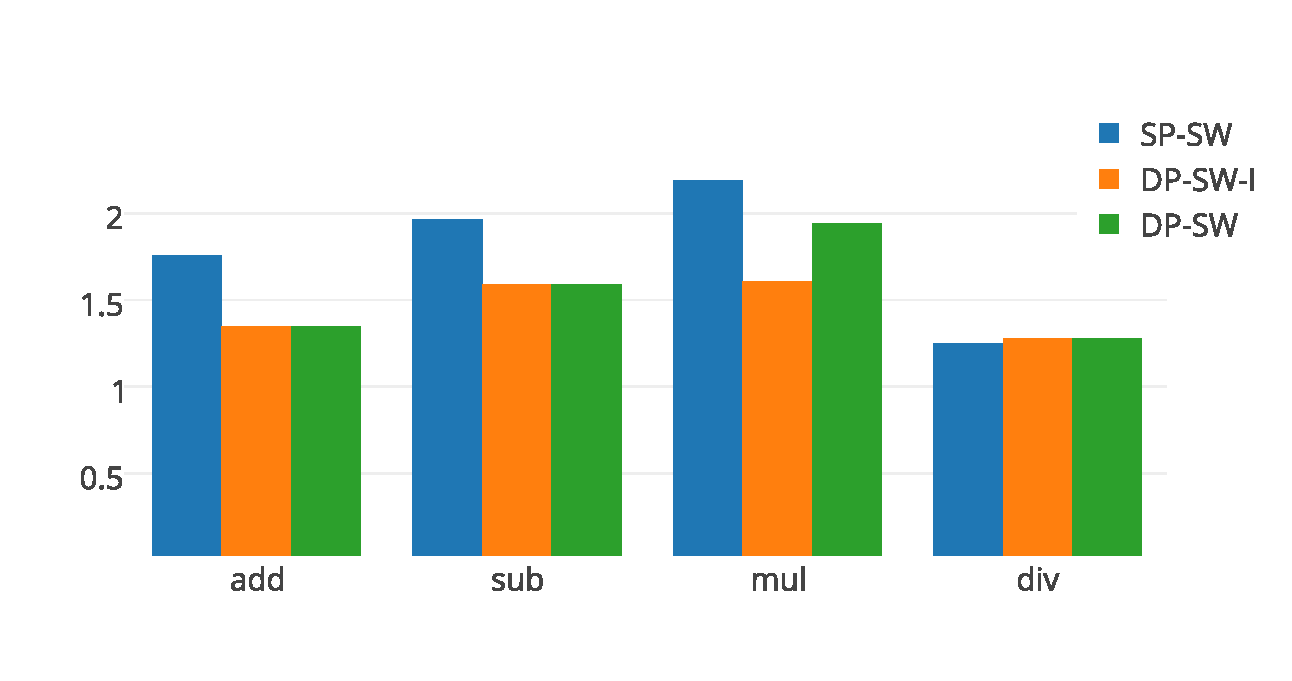
\includegraphics[scale=0.5]{ipetresults.pdf}
\caption{Current IPET analysis over-estimates WCET for software floating point operations compared.}
\label{f:ipetresults}
\end{figure}

This result has motivated the inclusion of FPUs in the cores. The FPU provided by Altera executes single precision operations using the custom instruction interface to the Nios II. Each instruction has a known execution time in clock cycles which eliminates the pessimism in calculating floating point operations. It is possible to force Simulink to generate code using only single precision variables and operations. There is a resulting tradeoff between the accuracy of the WCET estimation, the size of the core (inclusion of an FPU), and limiting calculations to single-precision. The FPU will also remove thousands of instructions from the critical function and reduce the interference due to instruction loads from main memory as well as lower execution time considerably. Future work on michro-architectural modelling may extend this analysis to several physical processors. Existing work on multicore WCET estimation is quite promising~\cite{chattopadhyay2014unified}.

\section{Stack Analysis}
It is possible to start analysis once the parser has built the CFG. Stack analysis is quite straightforward. Each basic block in a function is checked for instructions that increase the stack size. Note that stack instructions should not occur in a loop. If a basic block calls a function, then that function is also checked for stack instructions and then this result is added on to the original calculation. Recursive functions are not supported. Future work could analyze interrupt handlers as well to statically determine the maximum overhead due to interrupt handling.


\section{Library functions}

The object file and archive location of each library function has been determined and made statically available. There are (at least) two potential uses for this data. First, Some library functions may not conform to the patterns described in this Chapter. However, approximations based on runtime profiling could be substituted when library functions are encountered. Second, instruction prefetching into scratchpads requires that the entire call graph is known for the critical function. The library functions must be placed in a contiguous memory page for the simplistic virtual memory system currently implemented. Modifications to the linker script, a shown in Listing~\ref{l:jlib}, require the exact location for each function.

% 
\begin{lstlisting}[caption={Placing library functions in \texttt{.critical} region},label=l:jlib,language=C]
/* Library functions are: __muldf3,__muldi3,__pack_d,__unpack_d,__mulsi3,__lshrdi3,__ashldi3 */
/* To place these functions in a section called critical in linker.x: */
    .critical :
    {
        PROVIDE (_alt_partition_critical_start = ABSOLUTE(.));
        *(.critical .critical.*)

        /* INSERT THE FOLLOWING */

        */libgcc:_mul_df.o
        */libgcc:_unpack_df.o
        */libgcc:_pack_df.o
        */libgcc:_lshrdi3.o
        */libgcc:_ashldi3.o
        */libgcc:_muldi3.o
        */libgcc:lib2-mul.o

        /* END OF INSERTED CODED */

        . = ALIGN(4);

        PROVIDE (_alt_partition_critical_end = ABSOLUTE(.));
    } > processor0_0_scratchpad


\end{lstlisting}


